\documentclass[margin=3pt]{standalone}

\usepackage{tkz-euclide}

\begin{document}
	
	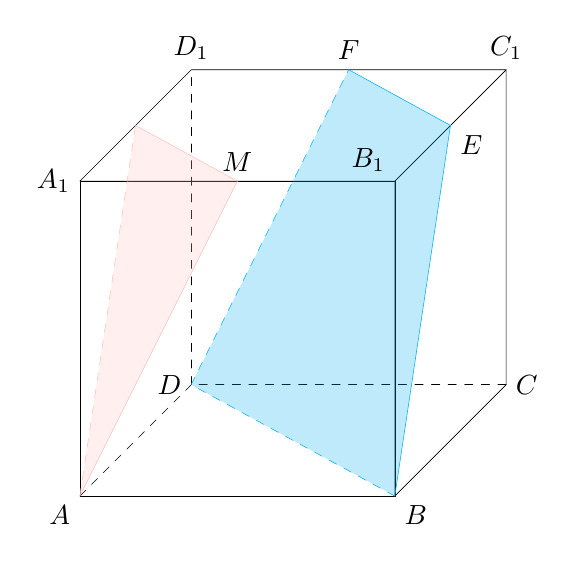
\begin{tikzpicture}[scale=1.00]
		\tkzInit
		\tkzDefPoint(3,4){A} % 起始点
		\edef\tkzLen{\fpeval{4}} % 边长
		\edef\tkzLenS{\fpeval{\tkzLen/2.0}}
		\tkzDefShiftPoint[A](0:\tkzLen cm){B}
		\tkzDefShiftPoint[A](45:\tkzLenS cm){D}
		\tkzDefSquare(A,B) \tkzGetPoints{B'}{A'}
		\tkzDefPointsBy[translation= from A to D](B,B',A'){C,C',D'}
		\tkzDefMidPoint(A',B') \tkzGetPoint{M}
		\tkzDefMidPoint(A',D') \tkzGetPoint{N}
		\tkzDefMidPoint(B',C') \tkzGetPoint{E}
		\tkzDefMidPoint(C',D') \tkzGetPoint{F}
		\tkzDrawPolygon(A,B,B',A')
		\tkzDrawPolygon(A',B',C',D')
		\tkzDrawPolygon(B,C,C',B')
		\tkzDrawSegments[dashed](A,D C,D D,D')
		\tkzDrawSegment[dashed,pink](A,N)
		\tkzDrawSegments[pink](A,M M,N)
		\tkzFillPolygon[pink,opacity=0.25](A,M,N)
		\tkzDrawSegments[dashed,cyan](D,F B,D)
		\tkzDrawSegments[cyan](B,E E,F)
		\tkzFillPolygon[cyan,opacity=0.25](B,E,F,D)
		\tkzLabelPoints[below left](A)
		\tkzLabelPoints[below right](B,E)
		\tkzLabelPoints[right](C)
		\tkzLabelPoints[left](D)
		\tkzLabelPoints[above](M,F)
		\tkzLabelPoint[left](A'){$A_1$}
		\tkzLabelPoint[above left](B'){$B_1$}
		\tkzLabelPoint[above](C'){$C_1$}
		\tkzLabelPoint[above](D'){$D_1$}
	\end{tikzpicture}
\end{document}

%%% Local Variables:
%%% mode: latex
%%% TeX-master: t
%%% End:
